\section{Theory}
\subsection{Membrane gas separation theory}
Hollow fiber membrane systems have somewhat the same configuration as tube and shell heat exchangers, as can be seen in \ref{fig:fig4}. The feed enters at one side of the membrane unit and flows through the tube or shell. While flowing through the tube, fluid will be permeated through the membrane walls. The remaining fluid leaving the membrane at the opposite end is called the retentate. The fluid that has permeated, the permeate, leaves the system through an outlet passage at either end of the membrane, depending on whether the configuration is counter-current (CC) or co-current (CO). 

\begin{figure}[H]
		\centering
	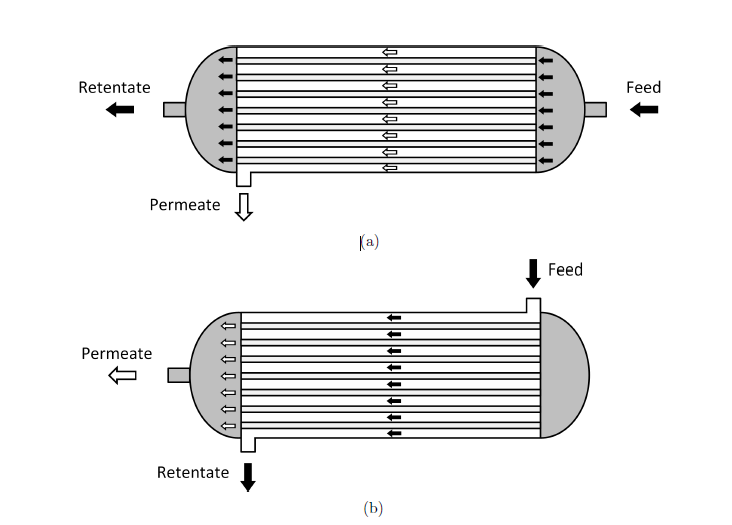
\includegraphics[width= 1\textwidth]{Images/fig7.png}
	\captionof{figure}{Representation of a hollow figer membrane setup; black arrows indicate fee/retentate flow, and white arrows indicate permeate flow: (a) bore feed, (b) shell feed \cite{Chourou2017}}
	\label{fig:fig4}
\end{figure}
The mass-flux over the membrane is controlled by $P_k$, the permeability of species $k$. The selectivity is given by the ratio of the permeabilities over the lowest permeability $\gamma_k = P_k/min\{P_k\}$. Low permeabilities lead typically to high selectivities and vice versa. \\
The physics related to gas separation is complicated since it depends on:
\begin{enumerate}
	\item the mass transfer mechanism across the membrane layer.
	\item  the flow pattern on the retentate and permeate side, which depends on; the pressure, velocity, species mass fraction and temperature. 
\end{enumerate}

\subsection{Discretization schemes}
In this section the central differencing scheme (CD), the upwind differencing scheme and the hybrid differencing scheme for a convection diffusion problem will be discussed as well as some properties of discretisation schemes. \\
 
Consider the one dimensional steady convection-diffusion equation for a general property $\phi$ in the absence of sources:
\begin{align}
&&	\frac{d}{dx} (\rho u \phi) = \frac{d}{dx}(\Gamma \frac{d \phi}{dx})
\end{align} 
The discretised convection-diffusion equation for the central, upwind and hybrid differencing schemes of a one-dimensional problem can be written as:
\begin{align}
&& a_P \phi_P = a_W\phi_W + a_E\phi_E	
\end{align}
with the coefficient of volume-cell 'P' as
\begin{align}
&&	a_P = a_W + a_E + (F_e-F_w)
\end{align}

\begin{figure}[H]
	\centering
	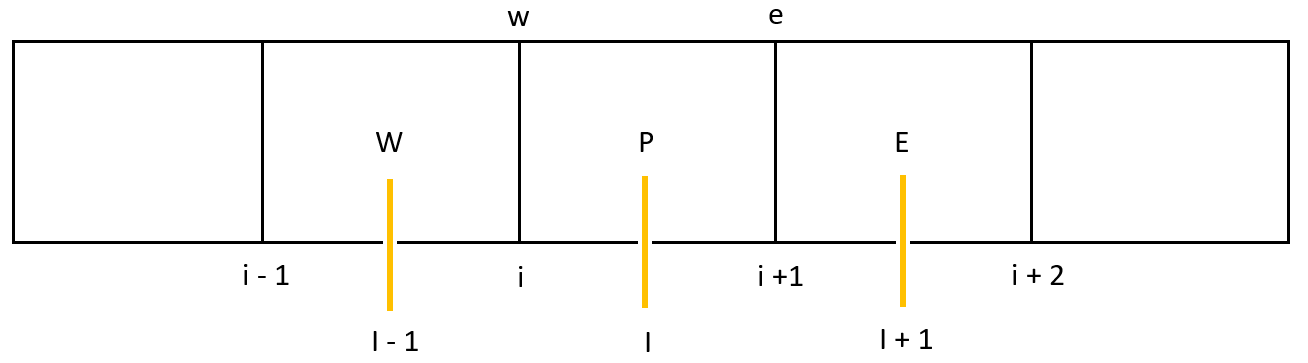
\includegraphics[width= 1\textwidth]{Images/fig1.png}
	\captionof{figure}{Discretised staggered grid.}
	\label{fig:fig6}
\end{figure}

The neighbour coefficients for these schemes are
\begin{table}[H]
	\centering
	\begin{tabular}{|l|l|l|}
		\hline
		Scheme &	$a_W$     & $a_E$   \\ \hline \vspace{-0.3cm}
		& & \\
		Central differencing & $D_w + \frac{F_w}{2}$  & $D_e - \frac{F_e}{2}$ \\ \hline \vspace{-0.3cm}
		& & \\
		Upwind differencing & $D_w + max\left[F_w, ,0\right]$  & $ D_e + max\left[0, -F_e\right]$ \\ \hline \vspace{-0.3cm}
		& & \\
		Hybrid differencing & $max\left[F_w, \left(D_w + \frac{F_w}{2}\right),0\right]$  & $max\left[-F_e, \left(D_e - \frac{F_e}{2}\right),0\right]$ \\ \hline
	\end{tabular}
\end{table}

In Figure \ref{fig:fig6} a schematic representation of the cell volumes is shown. \\

The boundary conditions enter the discretised equations via source terms. Their treatment is specific to each discretisation scheme. \\

Discretisation schemes that possess conservativeness, boundedness, and transportiveness give physically realistic results and stable iterative solutions. The central differencing method lacks transportiveness and gives unrealistic solutions for large values of the cell P\'eclet number. Hence it is not suitable for general-purpose convection-diffusion problems. Upwind and hybrid differencing schemes both possess conservativeness, boundedness and transportiveness and are highly stable, but suffer from false diffusion for multi-dimensional flows if the velocity vector is not parallel to one of the co-ordinate directions. In this work the hybrid scheme is preferred due to its stability and it has second order accuracy in terms of Taylor series for low $Pe$ numbers, $Pe < 2$.
 
\subsection{Numerical solver}
The discretization of equations is discussed in the previous section. This resulted in a system of linear algebraic equations which needs to be solved. The size and complexity of the system depends on the number of grid points, the discretisation method and the dimensionality of the problem. There exist two families of solution techniques for linear algebraic equations: \textbf{direct methods} and \textbf{indirect} or \textbf{iterative methods.}  %It is possible to determined the number op computations when using a direct method. The number of operations for a system of $N$ equations with $N$ unknowns solved by means of a direct method is of the order of $N^3$. A core memory of $N^2$ is required for the simultaneous storage of all coefficients of the set of equations. \\
This section only deals with the tri-diagonal matrix algorithm (TDMA), a direct method, and the Gauss-Seidel point-iterative method.  

\subsubsection{Gaus-Seidel}
The Gaus-Seidel method is a point-iterative algorithm and easy to implement. One condition for the iteration process to be convergent is that the matrix must be diagonally dominant. The finite volume method yields diagonally dominant systems as part of the discretisation process, so this aspect does not require special attention. The main disadvantage of this method is that the convergence rate can be slow when the system of equations is large. 
\subsubsection{TDMA}
The tri-diagonal matrix algorithm is a direct method for one-dimensional situations, but it can be applied iteratively to solve multi-dimensional problems. It consists of a forward elimination and back-substitution stage. This algorithm requires only a minimum amount of storage and is computationally inexpensive. 